\documentclass[11pt,a4paper]{scrarticle}
\usepackage[utf8]{inputenc}
\usepackage{cmap}
\usepackage[T2A]{fontenc}
\usepackage[russian]{babel}
\usepackage{amsmath,amssymb,amsthm,mathtools}
\usepackage{array}

\usepackage{indentfirst}
\usepackage{xcolor,graphicx, tikz, wrapfig}
\usepackage{longtable}
\usepackage{placeins}

% \usepackage{minted}
% \usemintedstyle{vs}

\usepackage[left=2cm,right=2cm,top=2cm,bottom=2cm,bindingoffset=0cm]{geometry}

\usepackage[unicode]{hyperref}
\definecolor{linkcolor}{HTML}{0000E6}
\definecolor{urlcolor}{HTML}{0000E6}
\definecolor{citecolor}{HTML}{0000E6}
\hypersetup{pdfpagemode=None,linktoc=page,citecolor=citecolor,linkcolor=linkcolor,urlcolor=urlcolor,colorlinks=true}

\theoremstyle{definition}
\newtheorem{subtask}{Пункт}

\DeclareMathOperator*{\argmax}{arg\,max}
\DeclareMathOperator*{\argmin}{arg\,min}
\newcommand{\floor}[1]{\left\lfloor #1 \right\rfloor}
\newcommand{\ceil}[1]{\left\lceil #1 \right\rceil}


\setlength{\parindent}{1cm}

\author{Клычков Максим Дмитриевич}

\begin{document}

\centerline{\textbf{\huge Алгоритмы и структуры данных-1}}
\centerline{\textbf{SET 3. Задача A1.}}
\begin{flushright}
	\emph{Осень 2024. Клычков М. Д.}
\end{flushright}

\begin{itemize}
	\item ID посылки по задаче \texttt{A1i}: \href{https://dsahse.contest.codeforces.com/group/NOflOR1Qt0/contest/565612/submission/292187460}{292187460}
	\item Ссылка на репозиторий:
\end{itemize}

Изначально был написан алгоритм Монте-Карло, генерирующий точки в широкой области, содержащей все три окружности. Эта область находилась с помощью нахождения минимумов/максимумов координат центров с прибавлением/вычитанием радиусов. Этот алгоритм прошел все тесты на \texttt{Codeforces}.

Затем на основе предыдущей программы была разработана новая, принимающая также параметры прямоугольной области для генерации точек. Вручную найдем область, максимально прилегающую к пересечению, при этом учтем, что операции с вещественными числами происходят не всегда точно, поэтому область будет расширена на величину $2\varepsilon \approx 0.02$ по $\epsilon \approx 0.01$ с каждой стороны.

\begin{figure}[htp]
	\centering
	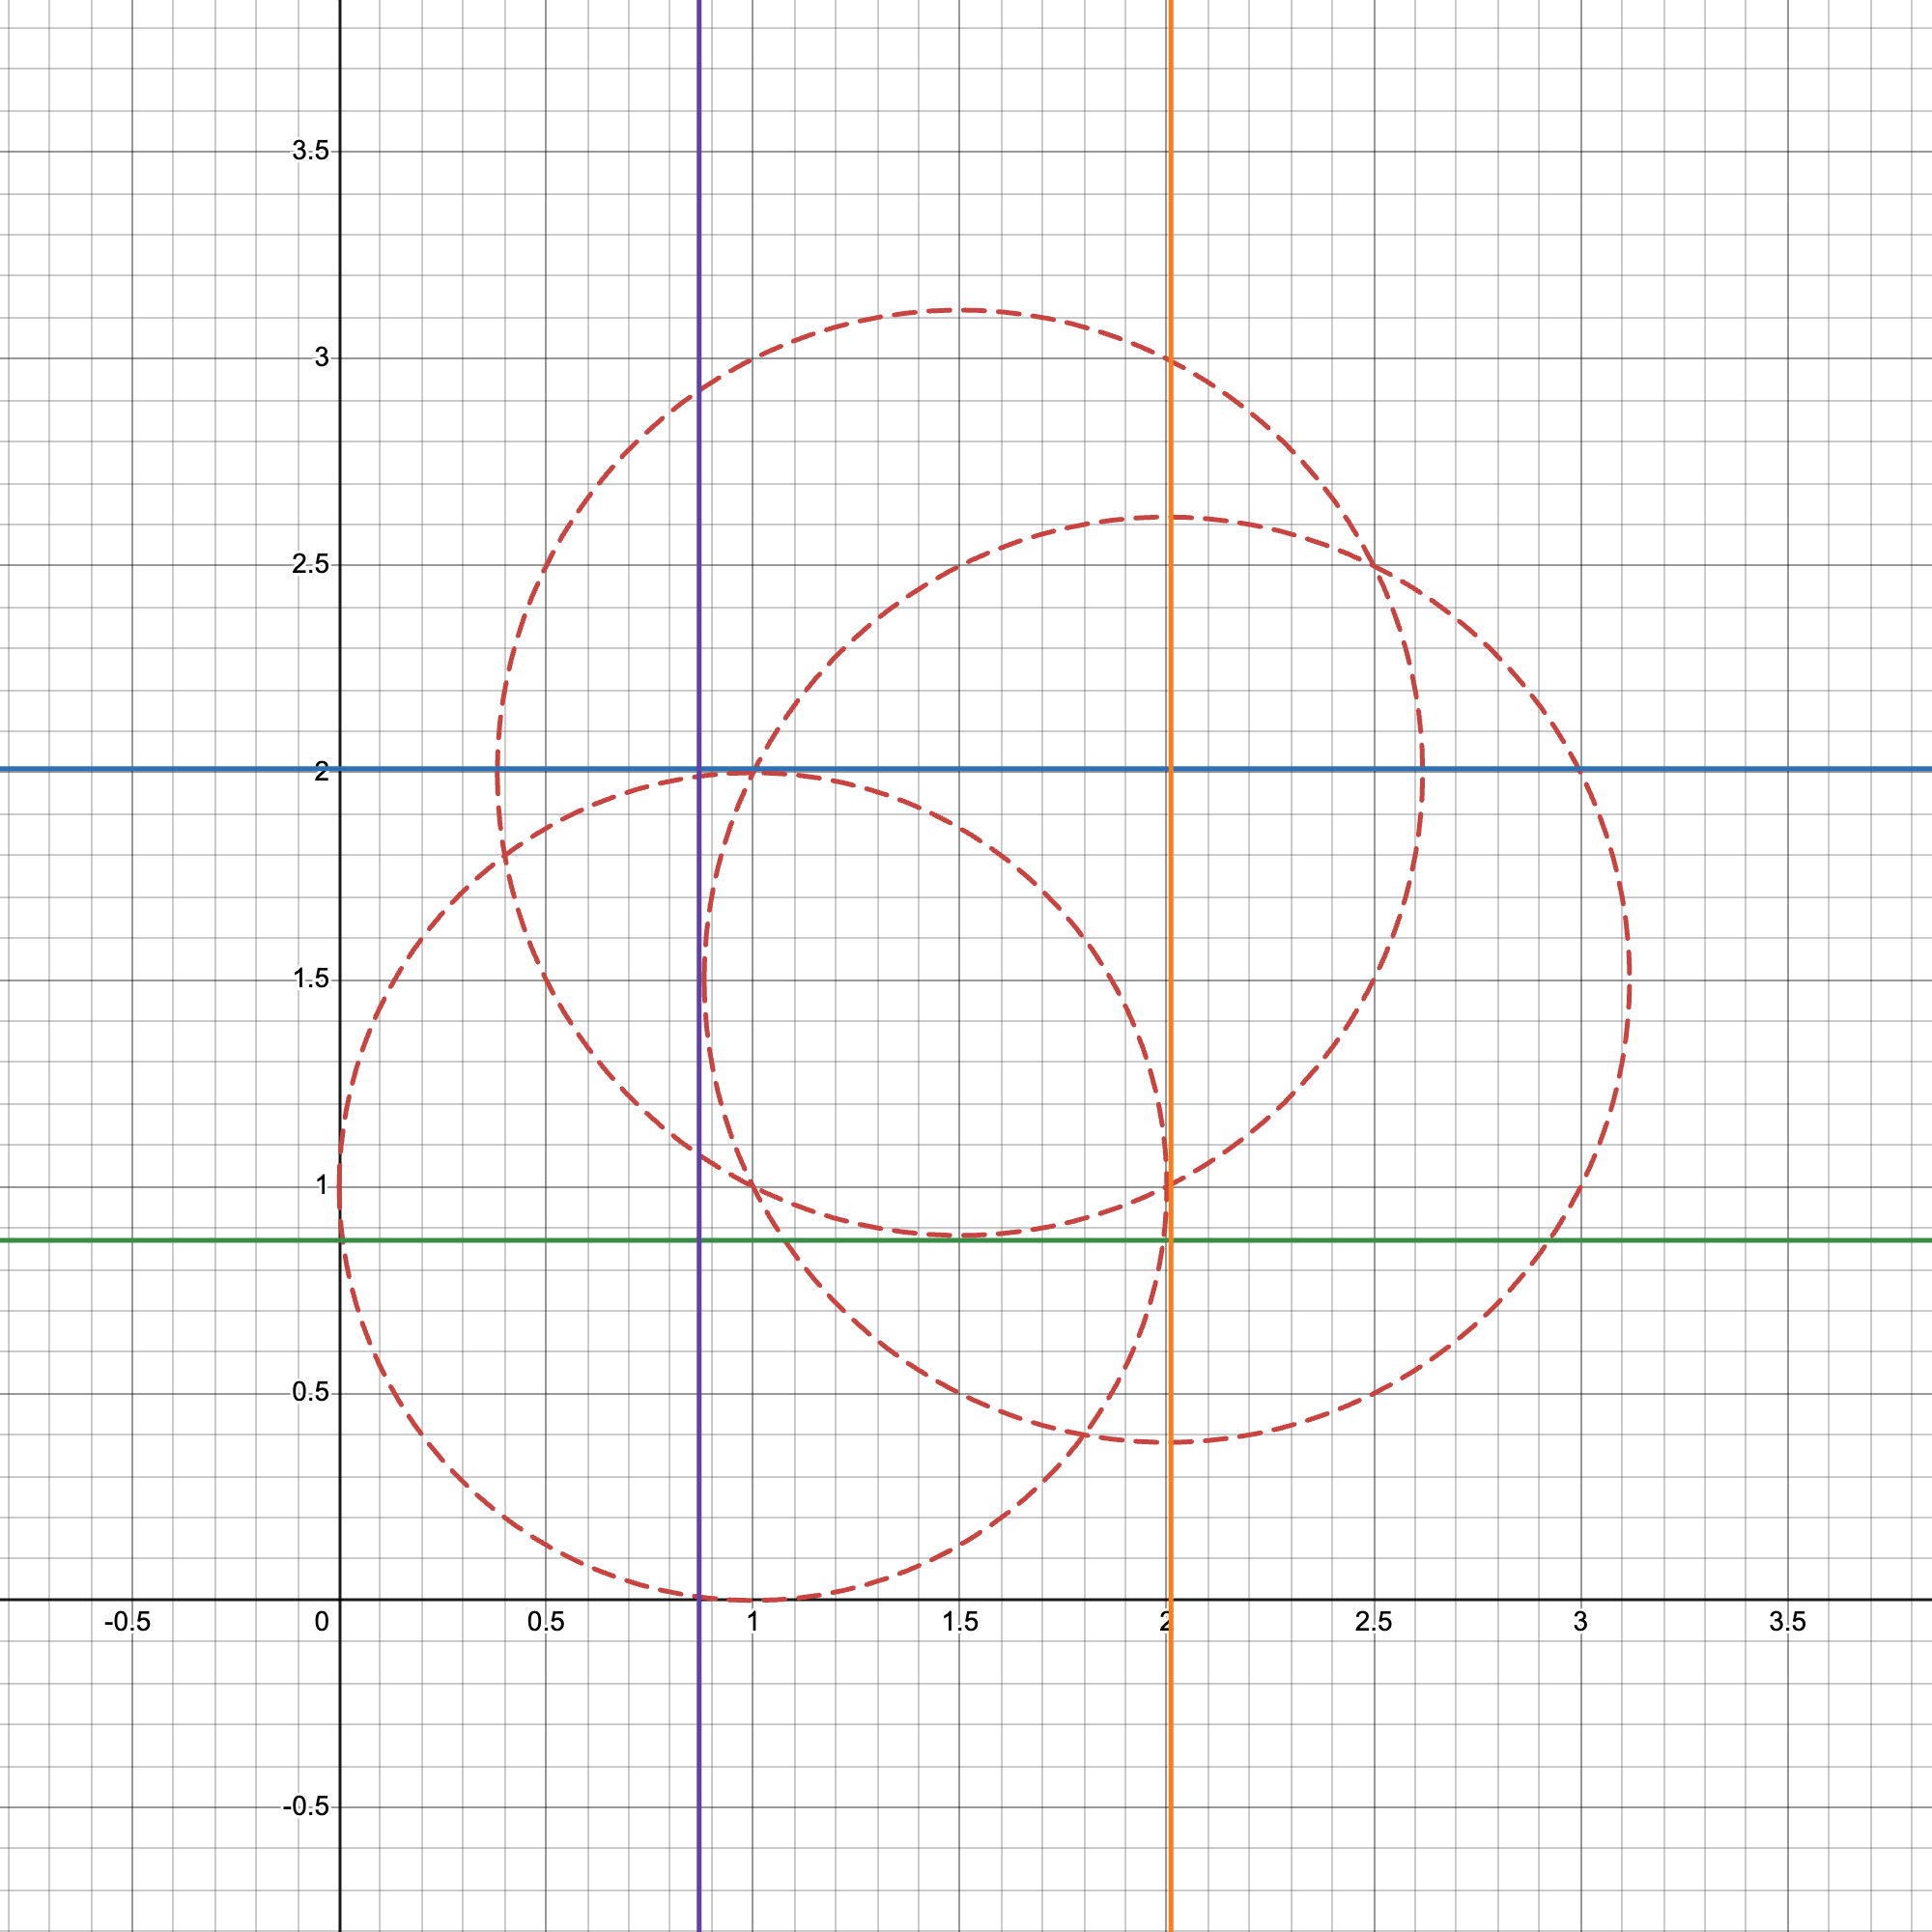
\includegraphics[width=0.5\textwidth]{../static/desmos-graph.png}
	\caption{Изображение «узкой» области генерации точек}
	\label{fig:desmos}
\end{figure}

Для экспериментальных запусков и построения графиков использовался язык \texttt{Python}.

\begin{enumerate}
	\item Графики первого типа, отображающие меняется приближенное значение площади в зависимости от количества сгенерированных точек. В одной системе координат были построены два графика, отличающихся областью генерации точек («широкой» и «узкой»).
	      \begin{figure}[htp]
		      \centering
		      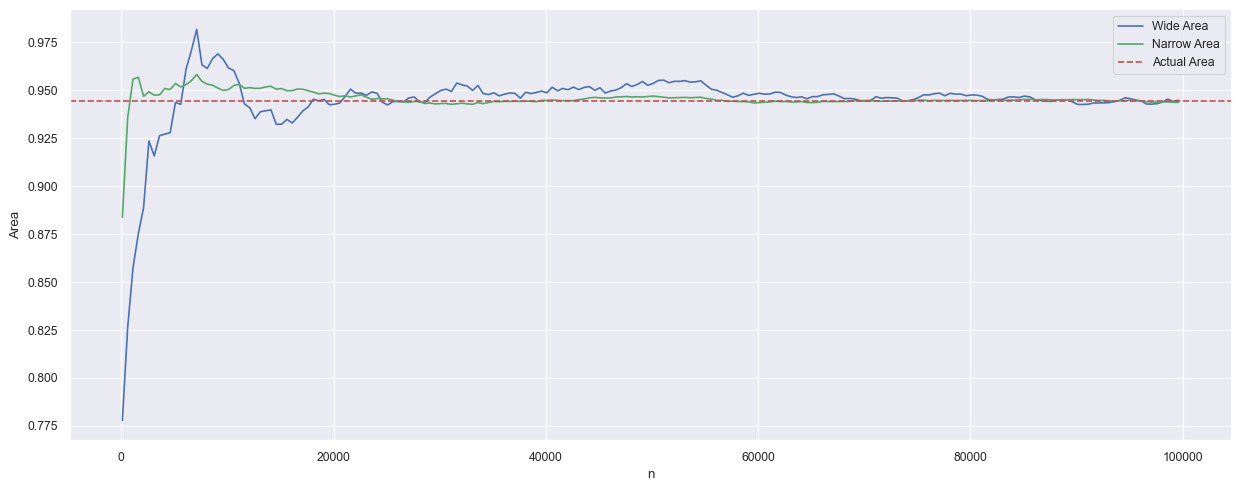
\includegraphics[width=\textwidth]{../static/area.png}
		      \caption{График первого типа}
		      \label{fig:area}
	      \end{figure}
	      \FloatBarrier

	      Полученные результаты начальных тестов не дают в полной мере оценить «хвост», поэтому изобразим без учета первых пяти результатов.
	      \begin{figure}[htp]
		      \centering
		      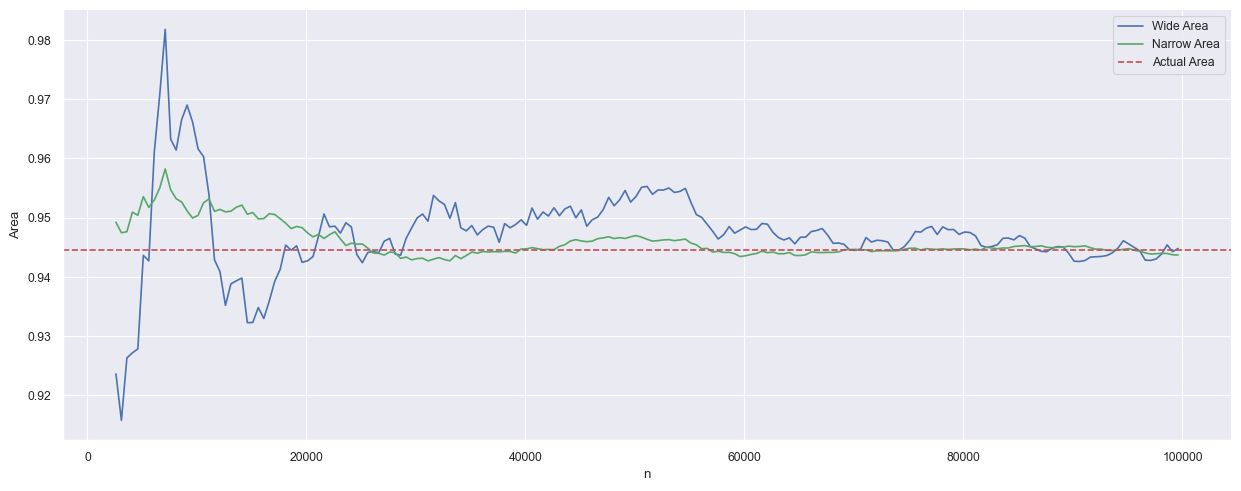
\includegraphics[width=\textwidth]{../static/area_reduced.png}
		      \caption{График первого типа без первых значений}
		      \label{fig:area-reduced}
	      \end{figure}
	      \FloatBarrier

	\item Графики второго типа, отображающие изменение величины относительного отклонения приближенного значения площади от ее точной оценки в зависимости от количества сгенерированных точек. Аналогично первому типу графиков будет отображены исходные данные и данные без первых нескольких значений.

	      \begin{figure}[htp]
		      \centering
		      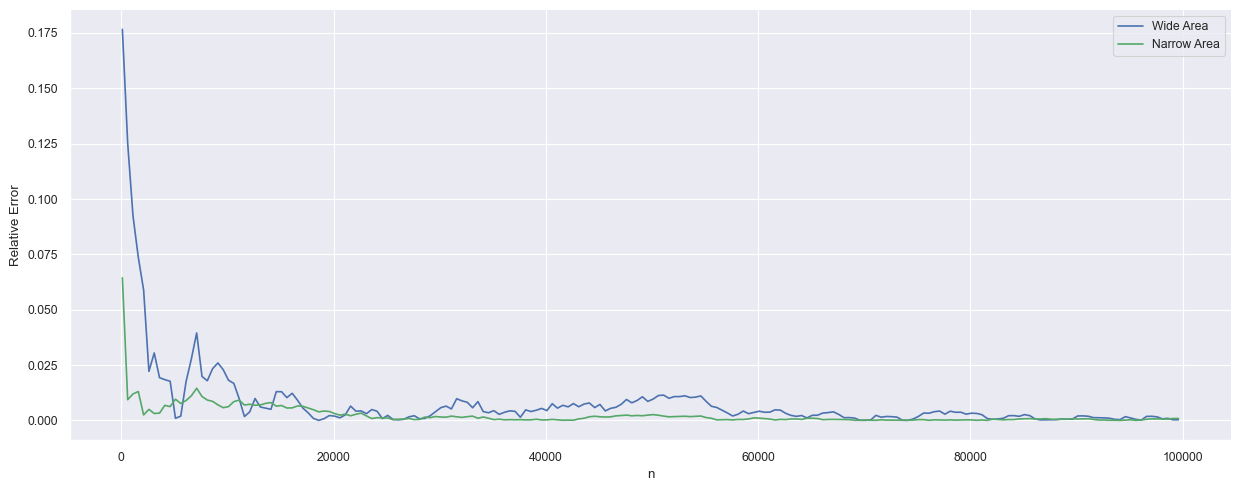
\includegraphics[width=\textwidth]{../static/relative_error.png}
		      \caption{График второго типа}
		      \label{fig:relative-error}
	      \end{figure}
	      \FloatBarrier

	      \begin{figure}[htp]
		      \centering
		      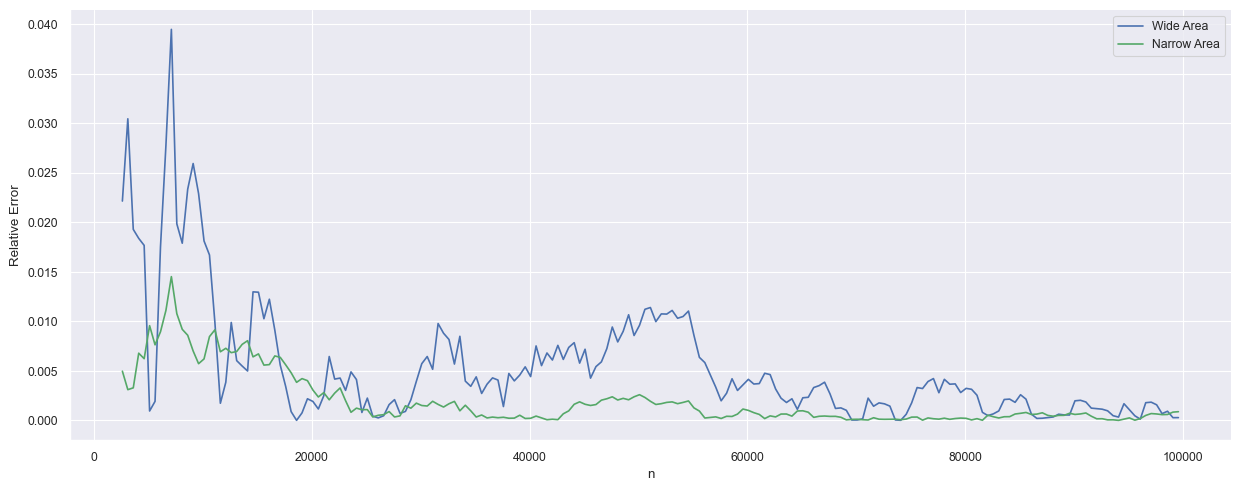
\includegraphics[width=\textwidth]{../static/relative_error_reduced.png}
		      \caption{График второго типа без первых значений}
		      \label{fig:relative-error-reduced}
	      \end{figure}
	      \FloatBarrier
\end{enumerate}

Перейдем к \textbf{выводам}:

\

В первую очередь отметим, что действительное значение площади фигуры, посчитанное по формуле из условия задачи $S \approx 0.9445171858994637$

Рассмотрим графики \emph{первого} типа. Заметим, что при малом числе сгенерированных точек наблюдаются большие колебания площади (до $n \approx 20000$), особенно они проявляются в алгоритме, учитывающем «широкую» область.

После указанного значения параметра $n$ зеленый график («узкая» область) начинает стабилизироваться около действительного значения площади фигуры (красная пунктирная линия), но в то же время оценка по «широкой» области продолжает вести себя неконтролируемо и при $n \approx 50000$ достигает значений площади $S_e \approx 0.955$, что отличается от действительного значения $|S_e - S| \approx 0.01$

В «хвосте» (по мере увеличения количества точек) приближенное значение площади стабилизируется, приближаясь к точной оценке, однако оценка по «узкой области» сильнее приближена к красной пунктирной линии фактического ответа.

\

Рассмотрим графики \emph{второго} типа. Графики построенные в одной системе координат явно демонстрируют, что относительное отклонение приближенного значения площади при генерации точек в «узкой» области почти всегда меньше, чем при генерации в «широкой» области.

Можно также заметить более менее монотонное убывание относительного отклонения зеленого графика, что совсем нельзя сказать про синий.

Относительное отклонение зеленого графика при достаточно больших значениях $n$ остается ниже $0.00025$, что свидетельствует о высокой точности результата.

\

На основе построенных графиков и сделанных выводов по ним можно утверждать, что для решения задачи оценки площади пересечения трех окружностей с высокой точностью следует использовать способ генерации точек в «узкой» области, однако он усложняется подбором границ области, который опускается в данном решении.

Тем не менее результат при способе генерации в «широкой» области также показывает удовлетворительные значения, которые например проходят тесты задачи в системе \texttt{Codeforces}.

\end{document}

